\documentclass[11pt,a4paper]{article}

\usepackage[utf8]{inputenc}
\usepackage[T1]{fontenc}
\usepackage{amsmath,amssymb,amsthm,amsfonts}
\usepackage{mathtools}
\usepackage{geometry}
\usepackage{graphicx}
\usepackage{booktabs}
\usepackage{hyperref}
\usepackage{algorithm}
\usepackage{algpseudocode}
\usepackage{natbib}
\usepackage{cleveref}
\usepackage{tikz}
\usetikzlibrary{positioning,arrows.meta,shapes.geometric,fit,backgrounds,trees}
\usepackage{xcolor}
\usepackage{bbm}

\geometry{margin=1in}

\newtheorem{theorem}{Theorem}[section]
\newtheorem{proposition}[theorem]{Proposition}
\newtheorem{lemma}[theorem]{Lemma}
\newtheorem{corollary}[theorem]{Corollary}
\theoremstyle{definition}
\newtheorem{definition}[theorem]{Definition}
\newtheorem{assumption}[theorem]{Assumption}
\theoremstyle{remark}
\newtheorem{remark}[theorem]{Remark}
\newtheorem{example}[theorem]{Example}

\DeclareMathOperator*{\argmin}{arg\,min}
\DeclareMathOperator*{\argmax}{arg\,max}
\newcommand{\R}{\mathbb{R}}
\newcommand{\N}{\mathbb{N}}
\newcommand{\Z}{\mathbb{Z}}
\newcommand{\E}{\mathbb{E}}
\renewcommand{\Pr}{\mathbb{P}}
\newcommand{\Sc}{\mathcal{S}}
\newcommand{\Qc}{\mathcal{Q}}
\newcommand{\Tc}{\mathcal{T}}
\newcommand{\Cc}{\mathcal{C}}
\newcommand{\Mc}{\mathcal{M}}
\newcommand{\Rc}{\mathcal{R}}

\title{Hierarchical Navigation Cascades:\\
Sub-Linear Question Routing Through\\
Specialist Partition Trees}

\author{Kundai Farai Sachikonye\\
\texttt{kundai.sachikonye@wzw.tum.de}}

\date{\today}

\begin{document}
\maketitle

\begin{abstract}
Contemporary language-model-based systems confront a scaling paradox: capabilities improve with parameter count, but inference cost grows proportionally, and every query pays the full cost regardless of difficulty. A simple arithmetic question invokes the same inference pipeline as a complex analytical one. We develop an alternative architecture in which a large ensemble of \emph{specialist} language models --- each small, each trained on a narrow task --- is organized into a $k$-ary partition tree, and incoming questions are routed through the tree in $O(\log_k N)$ model invocations, where $N$ is the number of leaf specialists. Each invocation is on a small model of fixed capacity; the total inference cost per query is therefore $O(\log_k N \cdot |\theta_{\text{small}}|)$, which can be orders of magnitude below the cost of a monolithic model that matches the ensemble's aggregate capability. We prove that the routing problem is itself a bounded-depth classification task whose capacity requirements are independent of leaf specialist complexity, and we establish a self-similarity result: the same routing primitive operates at multiple scales, permitting specialists at one level to serve as routers at a finer level without architectural change. The self-similarity yields an \emph{additive} latency bound --- $\sum_i O(\log_{k_i} N_i)$ across scales --- rather than the multiplicative bound naive analyses might suggest. We analyze the economics of capability addition, prove a failure-localization property, and specify validation protocols. The architecture implies a reorientation of where model scale is spent: not in a single monolithic parameter matrix, but distributed across a hierarchy of small, independently updatable models indexed by a routing tree.
\end{abstract}

\section{Introduction}
\label{sec:intro}

\subsection{The Scaling Paradox}

The prevailing trajectory in language model development is to increase capability by increasing parameter count \citep{kaplan2020scaling, hoffmann2022training}. A model with more parameters generalizes better and handles a wider range of tasks. Its inference cost, however, is proportional to the parameter count, and this cost is paid for every query regardless of whether the query exploits the model's breadth.

In production deployments, the paradox manifests sharply. Answering ``what is the capital of France'' and answering ``write a proof that every finite group has a subgroup of prime order'' both invoke the full model. The former could be answered by a far smaller specialized system, but the cost of maintaining many small systems --- training, deployment, routing, fallback --- has historically exceeded the cost of simply using a large general-purpose model.

This paper develops an architecture that changes the cost balance. We propose organizing specialist models into a hierarchical tree, and routing questions through the tree with $O(\log_k N)$ small-model invocations where $N$ is the number of specialists and $k$ the tree branching factor. Crucially, the routing itself is a small-model task, not a large one: routing decisions are $k$-way classifications at each level, which we prove can be carried out with capacity independent of specialist size.

\subsection{The Cascade Alternative}

The architecture has three components:

\begin{enumerate}
    \item A \emph{specialist tree}: a rooted $k$-ary tree whose leaves are small expert models, each specialized to a narrow task, and whose internal nodes are routing classifiers.
    \item A \emph{routing protocol}: for each incoming question, descend the tree from root to leaf, invoking the router at each internal node to select the appropriate child.
    \item An \emph{answering protocol}: at the leaf, the specialist model produces the answer.
\end{enumerate}

For a tree of depth $D = \log_k N$ with $N$ leaves, a query invokes $D$ routers plus one leaf specialist. If each router and each specialist is a model of fixed size $|\theta_s|$, the total inference cost is $(D + 1) |\theta_s| = O(\log_k N \cdot |\theta_s|)$.

\subsection{Why This Is Not Obvious}

A natural objection: routing is itself a difficult task. If a small router cannot distinguish between the expertise of two child subtrees, the cascade's output quality will be bounded by router error.

We address this objection directly. The routing task at each internal node is a $k$-way classification over the space of queries. Its difficulty is governed by the \emph{granularity} of distinctions the router must make, not by the sophistication of the leaf specialists. A router deciding between ``mathematical-query subtree'' and ``literary-query subtree'' needs to recognize mathematical notation, algebraic manipulation requests, etc.; it does not need to solve the mathematical problem itself.

We show (Section~\ref{sec:routing-complexity}) that routing capacity scales with the classification granularity, not with specialist expertise. This is what makes the cascade architecture feasible.

\subsection{Contributions}

\begin{enumerate}
    \item A formal specification of the specialist partition tree (Section~\ref{sec:tree}).
    \item A complexity result for routing through the tree ($O(\log_k N)$ invocations of bounded-capacity routers, Section~\ref{sec:routing-complexity}).
    \item A self-similarity result: the routing primitive is scale-invariant, so specialists can nest as routers at a finer scale without architectural change (Section~\ref{sec:self-similar}).
    \item An additive-latency theorem: end-to-end latency across multiple scales is $\sum_i O(\log_{k_i} N_i)$, not $\prod_i O(\log_{k_i} N_i)$ (Section~\ref{sec:multi-scale}).
    \item Failure-localization: bounded propagation of specialist-level errors (Section~\ref{sec:failure}).
    \item An economic analysis of capability scaling via specialist addition vs.\ parameter addition (Section~\ref{sec:economics}).
    \item A distillation protocol for generating specialist models from a more general teacher (Section~\ref{sec:distillation}).
    \item Validation protocols for each theoretical claim (Section~\ref{sec:validation}).
\end{enumerate}

\subsection{Organization}

Section~\ref{sec:preliminaries} fixes notation.
Section~\ref{sec:problem} formalizes the routing problem.
Section~\ref{sec:tree} defines the specialist partition tree.
Section~\ref{sec:routing-complexity} proves the sub-linear routing bound.
Section~\ref{sec:self-similar} establishes self-similarity.
Section~\ref{sec:multi-scale} extends to multi-scale stacks.
Section~\ref{sec:failure} analyzes failure modes.
Section~\ref{sec:economics} analyzes capability economics.
Section~\ref{sec:distillation} discusses training.
Section~\ref{sec:validation} specifies experiments.
Section~\ref{sec:related} surveys related work.
Section~\ref{sec:discussion} discusses implications.
Section~\ref{sec:conclusion} concludes.

\section{Preliminaries}
\label{sec:preliminaries}

\subsection{Questions and Answers}

Let $\Qc$ be a countable set of \emph{questions}. Each question is a finite sequence of tokens drawn from an alphabet $\Sigma$. Let $\mathcal{A}$ be a countable set of \emph{answers}, similarly structured. A $\emph{question-answering system}$ is a (possibly randomized) function $S: \Qc \to \mathcal{A}$.

We assume a reference distribution $\Pr_{\star}$ over $(q, a)$ pairs reflecting the intended behaviour. The \emph{error rate} of $S$ is $\Pr_{(q,a) \sim \Pr_{\star}}[S(q) \neq a]$.

\subsection{Models as Answering Systems}

A \emph{model} is an answering system implemented as a parameterized function $f_\theta: \Qc \to \mathcal{A}$, with parameter vector $\theta \in \R^p$. The \emph{capacity} of the model is $|\theta| = p$.

Inference cost on a single question is $\Theta(|\theta|)$ floating-point operations, up to constants depending on the model architecture.

\subsection{$k$-Ary Trees}

A \emph{$k$-ary tree} is a rooted tree in which every internal node has exactly $k$ children. For a balanced $k$-ary tree of depth $D$, the number of leaves is $N = k^D$, and the depth is $D = \log_k N$.

We associate each internal node with a \emph{router} and each leaf with a \emph{specialist}. We write $\mathcal{T} = (V, E)$ for the tree with vertices $V$ partitioned into internal nodes $V_I$ and leaves $V_L$, and edges $E$ directed from parent to child.

\section{The Question Routing Problem}
\label{sec:problem}

\subsection{Problem Statement}

Given an ensemble of $N$ specialist models $\{f_i\}_{i=1}^N$, each with domain of competence $\mathcal{Q}_i \subseteq \Qc$, we wish to build an answering system that routes each incoming question $q$ to the specialist whose competence domain contains $q$.

Formally, let $\rho: \Qc \to \{1, \ldots, N\}$ be the \emph{ideal routing function} that assigns each question to the specialist best suited to answer it. An approximate router $\hat\rho$ induces the answering system
\[
S_{\hat\rho}(q) \;=\; f_{\hat\rho(q)}(q).
\]
The error rate of $S_{\hat\rho}$ decomposes as
\[
\mathrm{err}(S_{\hat\rho}) \;\leq\; \mathrm{err}(\hat\rho) + \max_i \mathrm{err}(f_i \mid \mathcal{Q}_i),
\]
where the first term is routing error and the second is specialist error.

\subsection{Naive Routing}

The simplest router is an $N$-way classifier that takes a question and outputs one of $N$ specialist indices. Its capacity must scale with $N$ (at least $\log_2 N$ output bits) and its inference cost is $\Theta(|\theta_{\mathrm{naive}}|)$ per query.

For small $N$ this is acceptable. For large $N$, the naive router becomes the bottleneck: a system with $10^5$ specialists requires a $\log_2 10^5 \approx 17$-bit output router, which in practice is a substantial classifier with tens to hundreds of millions of parameters. Moreover, adding a specialist requires retraining the $N$-way classifier.

\subsection{Hierarchical Routing}

The hierarchical alternative replaces the single $N$-way classifier with a tree of $k$-way classifiers. The tree has $\lceil \log_k N \rceil$ levels; at each level, a $k$-way classifier selects one of $k$ subtrees. After $\lceil \log_k N \rceil$ levels the leaf specialist is reached.

\begin{figure}[t]
\centering
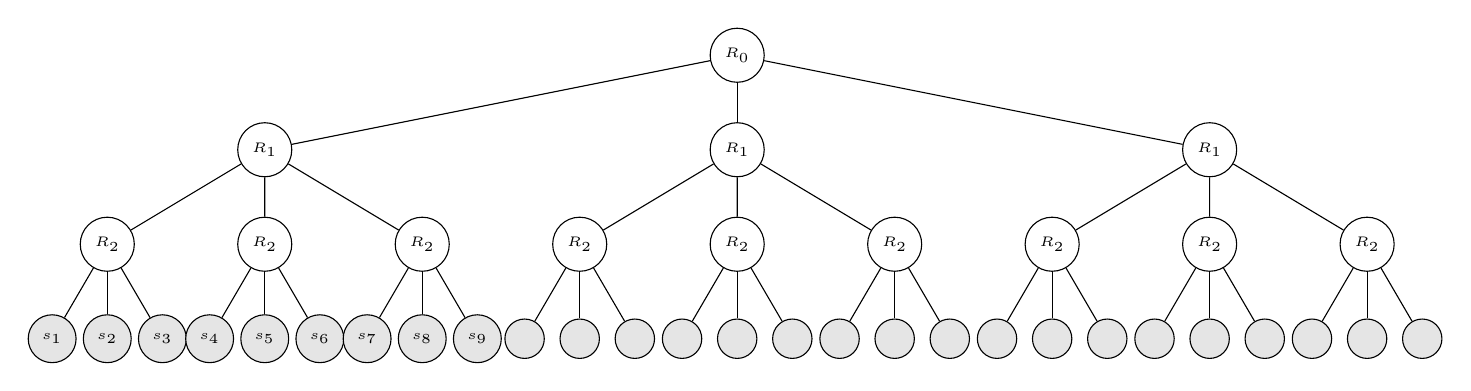
\begin{tikzpicture}[
  level distance=1.2cm,
  level 1/.style={sibling distance=6cm},
  level 2/.style={sibling distance=2cm},
  level 3/.style={sibling distance=0.7cm},
  every node/.style={draw, circle, minimum size=6mm, font=\tiny},
  leaf/.style={draw, circle, minimum size=5mm, fill=gray!20, font=\tiny}]

\node {$R_0$}
  child { node {$R_1$}
    child { node {$R_2$}
      child { node[leaf] {$s_1$} }
      child { node[leaf] {$s_2$} }
      child { node[leaf] {$s_3$} }
    }
    child { node {$R_2$}
      child { node[leaf] {$s_4$} }
      child { node[leaf] {$s_5$} }
      child { node[leaf] {$s_6$} }
    }
    child { node {$R_2$}
      child { node[leaf] {$s_7$} }
      child { node[leaf] {$s_8$} }
      child { node[leaf] {$s_9$} }
    }
  }
  child { node {$R_1$}
    child { node {$R_2$} child{ node[leaf]{} } child{ node[leaf]{} } child{ node[leaf]{} }}
    child { node {$R_2$} child{ node[leaf]{} } child{ node[leaf]{} } child{ node[leaf]{} }}
    child { node {$R_2$} child{ node[leaf]{} } child{ node[leaf]{} } child{ node[leaf]{} }}
  }
  child { node {$R_1$}
    child { node {$R_2$} child{ node[leaf]{} } child{ node[leaf]{} } child{ node[leaf]{} }}
    child { node {$R_2$} child{ node[leaf]{} } child{ node[leaf]{} } child{ node[leaf]{} }}
    child { node {$R_2$} child{ node[leaf]{} } child{ node[leaf]{} } child{ node[leaf]{} }}
  };

\end{tikzpicture}
\caption{A ternary specialist tree of depth 3 with 27 leaf specialists. Each internal node $R_i$ is a routing classifier selecting among its three children. Path length from root to any leaf is $\log_3 27 = 3$.}
\label{fig:tree}
\end{figure}

The hierarchical router's total inference cost is the sum of the per-level router costs plus the specialist cost. If each router has capacity $|\theta_r|$ and each specialist $|\theta_s|$, total inference is $\log_k N \cdot |\theta_r| + |\theta_s|$, which we now analyze.

\section{Specialist Partition Trees}
\label{sec:tree}

\subsection{Construction}

Given a set of $N$ specialists with a relation of \emph{semantic similarity} (e.g., two specialists are similar if they cover overlapping subsets of $\Qc$), we construct the specialist tree recursively:

\begin{algorithm}
\caption{Build Specialist Tree}
\label{alg:build}
\begin{algorithmic}[1]
\Function{BuildTree}{$\Mc$, $k$}
    \If{$|\Mc| \leq k$}
        \State \Return Leaf node with specialists $\Mc$
    \EndIf
    \State Partition $\Mc$ into $k$ clusters $\Mc_1, \ldots, \Mc_k$ by semantic similarity
    \State Train router $R$ on labeled questions, where a question is labeled with cluster index $j$ if its ideal specialist is in $\Mc_j$
    \State \Return Internal node with $R$ and children $\Call{BuildTree}{\Mc_j, k}$ for each $j$
\EndFunction
\end{algorithmic}
\end{algorithm}

The clustering in Step 4 is the critical design choice. A good clustering is one where (i) clusters are small enough to be further refined recursively, (ii) the boundary between clusters corresponds to a recognizable distinction in question space, and (iii) clusters are balanced so tree depth is minimized.

\subsection{Design Invariants}

We impose two invariants on the constructed tree:

\begin{definition}[Tree Invariants]
\label{def:invariants}
A specialist partition tree $\Tc$ satisfies:
\begin{enumerate}
    \item \textbf{Locally $k$-way balanced}: every internal node has between $\lceil k/2 \rceil$ and $k$ children.
    \item \textbf{Globally depth-balanced}: leaves are at depths differing by at most one.
\end{enumerate}
\end{definition}

Invariant 1 ensures the branching factor is close to $k$; invariant 2 ensures the tree is within $O(1)$ of balanced. Standard balancing techniques (e.g., weight-balanced partitioning) achieve both.

\subsection{Alternatives to Fixed Branching Factor}

A fixed $k$ is not essential. Variable-branching trees (e.g., adapting $k$ to local semantic clustering) yield better empirical clusters in some domains. Our theoretical results are stated for fixed $k$ for clarity but extend to variable branching with bounded $k_{\max}$.

\section{Routing Complexity}
\label{sec:routing-complexity}

\subsection{Per-Level Routing as Classification}

At each internal node, routing is a $k$-way classification: given a question $q$, output one of $k$ subtree indices. This is a standard classification problem. We characterize its capacity.

\begin{assumption}[Bounded Local Separability]
\label{assum:sep}
At each internal node $v$ at depth $d$, the ideal routing function $\rho_v: \Qc \to \{1, \ldots, k\}$ admits a classifier with error $\varepsilon_d > 0$ using capacity $|\theta_r(d)| \leq C_r \cdot \log_2 k \cdot \mathrm{poly}(1/\varepsilon_d)$, where $C_r$ is a constant depending on the embedding geometry but not on the depth $d$ or the subtree content.
\end{assumption}

Assumption~\ref{assum:sep} is the key non-trivial condition. It asserts that the granularity of distinction at each level is bounded --- routers at every level solve a problem of comparable difficulty. This is plausible because each level halves (actually divides by $k$) the remaining question space; the distinctions required are ever finer, but each is only among $k$ options.

\subsection{Main Theorem}

\begin{theorem}[Routing Complexity]
\label{thm:route-complexity}
Under Assumption~\ref{assum:sep} and a balanced specialist partition tree with $N$ leaves and branching factor $k$:
\begin{enumerate}
    \item The number of router invocations per query is $\log_k N + O(1)$.
    \item The total router capacity along any root-to-leaf path is $O(\log_k N \cdot \log_2 k \cdot \mathrm{poly}(1/\bar\varepsilon))$, where $\bar\varepsilon = \min_d \varepsilon_d$ is the worst per-level error rate.
    \item The total inference cost per query is
    \[
    T_{\text{infer}} \;=\; O\!\left( \log_k N \cdot |\theta_r| + |\theta_s| \right),
    \]
    where $|\theta_r|$ is the per-level router capacity and $|\theta_s|$ is the leaf specialist capacity.
\end{enumerate}
\end{theorem}

\begin{proof}
Part 1 is immediate from the tree balance. The path from root to any leaf has length at most $\lceil \log_k N \rceil + 1$ (the $+1$ accounting for within-leaf index lookup).

Part 2 follows by summing per-level capacities from Assumption~\ref{assum:sep} along the path.

Part 3 sums the router and specialist inference costs.
\end{proof}

\begin{corollary}[Sub-Linear Routing]
\label{cor:sublinear}
For fixed router capacity $|\theta_r|$ and specialist capacity $|\theta_s|$, inference cost per query grows only logarithmically in the number of specialists:
\[
T_{\text{infer}}(N) \;=\; O(\log N).
\]
\end{corollary}

\subsection{Aggregate System Capability}

The cascade's aggregate capability is the union of specialist capabilities. If each specialist has capacity $|\theta_s|$ and covers a competence domain $\mathcal{Q}_i$, the system covers $\bigcup_i \mathcal{Q}_i$.

For an ensemble with $N$ specialists each of capacity $|\theta_s|$, the total parameter count is $N \cdot |\theta_s|$ at leaves plus $\log_k N \cdot |\theta_r|$ at routers, giving aggregate $N \cdot |\theta_s| + \log_k N \cdot |\theta_r|$.

The comparison with a single model of aggregate capacity $|\theta_{\text{mono}}| = N \cdot |\theta_s|$ is striking: the cascade and monolith have comparable total parameters, but inference cost per query is $O(\log N)$ vs.\ $O(N)$ times the per-model factor. For $N = 1000$ and $k = 3$, the cascade pays approximately $7$ small-model inferences per query, while a monolithic model matching the aggregate capacity pays $1000$ times a small-model inference.

\begin{remark}[Amortization across queries]
The monolithic comparison assumes the monolith cannot reuse computation across queries. If weight sharing and cache reuse lower the effective per-query cost of a large model (as transformer architectures permit), the cascade advantage diminishes. The cascade retains its $O(\log N)$-vs-$O(|\theta_{\text{mono}}|)$ advantage when queries are independent and diverse, which is the realistic setting for an open-ended natural-language interface.
\end{remark}

\subsection{Router Error Propagation}

Errors compound along the routing path. If each per-level router has error $\varepsilon_r$, the probability that all $\log_k N$ routing decisions are correct is $(1 - \varepsilon_r)^{\log_k N}$. For small $\varepsilon_r$,
\[
\Pr[\text{correct routing}] \;\approx\; 1 - \varepsilon_r \log_k N.
\]

\begin{proposition}[Path Error Bound]
\label{prop:path-error}
In a depth-$D$ cascade where each router has error probability at most $\varepsilon_r$ and specialists have error $\varepsilon_s$, the system's error rate is at most
\[
\varepsilon_{\text{sys}} \;\leq\; \varepsilon_r \cdot D + \varepsilon_s.
\]
\end{proposition}

\begin{proof}
Union bound over the $D$ router decisions plus the specialist.
\end{proof}

To keep $\varepsilon_{\text{sys}} \leq \varepsilon_{\text{target}}$, per-level router error should be $\varepsilon_r \leq (\varepsilon_{\text{target}} - \varepsilon_s) / D$, which is mild for practical $D \leq 30$.

\section{Self-Similarity and Scale Invariance}
\label{sec:self-similar}

\subsection{Scale-Invariance of the Routing Primitive}

The routing primitive --- ``$k$-way classify a question into the appropriate subtree'' --- is the same operation at every depth of the tree. This is not accidental. It follows from the hierarchical construction: each subtree is itself a specialist tree, of smaller size but the same structure.

\begin{proposition}[Sub-Tree Self-Similarity]
\label{prop:selfsim}
Any depth-$d$ subtree of a balanced specialist partition tree $\Tc$ of depth $D$ is itself a specialist partition tree of depth $D - d$, with the same branching factor and invariants.
\end{proposition}

\begin{proof}
By construction: Algorithm~\ref{alg:build} recursively partitions until the specialist set fits in a leaf. Any intermediate call produces a tree that satisfies the invariants for its depth.
\end{proof}

\subsection{Specialists as Routers at Lower Scales}

The self-similarity has a strong architectural consequence: a specialist at one scale can serve as a router at a lower scale, without any architectural change.

\begin{definition}[Dual-Role Model]
A dual-role model is a parameter vector $\theta$ that functions as both a leaf specialist (answering questions in its domain) and as a router (classifying questions to appropriate sub-specialists of its domain).
\end{definition}

Concretely: a model trained to answer ``chemistry'' questions may also be used to route ``chemistry'' questions to an inner tree of ``organic'', ``inorganic'', ``physical'' sub-specialists. The same model can act as both the answer-generator for general chemistry and the router for specialized chemistry.

\begin{theorem}[Scale-Invariance of Architecture]
\label{thm:scale-inv}
There exists no architectural distinction between routers at different levels of the tree. A router trained for depth-$d$ classification has the same architecture (up to parameter count) as a router at depth-$d'$ for any $d, d'$.
\end{theorem}

\begin{proof}
Routers at every level perform $k$-way classification on questions. The input space is the same ($\Qc$), the output space is the same ($\{1, \ldots, k\}$), and the training procedure is the same (supervised classification over labelled routing data). No depth-dependent architecture is required.
\end{proof}

The practical implication is significant: a router can be promoted from operating at depth $d$ to depth $d-1$ (to serve a larger question space) by retraining with new labelled data, without modifying its architecture. Dually, a specialist at a leaf can be ``extended'' into a subtree by adding a few finer-grained sub-specialists and retraining the specialist to serve as their router.

\section{Multi-Scale Stacks}
\label{sec:multi-scale}

\subsection{Multiple Routing Stages}

Real systems may route through multiple stages, each performing a different kind of classification. For instance:
\begin{enumerate}
    \item \textbf{Domain routing}: ``is this question about biology, chemistry, or computer science?''
    \item \textbf{Sub-domain routing}: within biology, ``is this about molecular, cellular, or organismal?''
    \item \textbf{Specific-specialist routing}: within molecular biology, ``is this about DNA, RNA, or proteins?''
\end{enumerate}

Each stage is a specialist tree. The end-to-end pipeline is a sequence of trees, each resolving one layer of the question.

\subsection{Additive Latency}

A naive analysis might suggest that multi-stage routing incurs multiplicative latency: if stage $i$ has $N_i$ leaves, total invocations are $\prod_i \log_{k_i} N_i$. This is wrong.

\begin{theorem}[Additive Multi-Scale Latency]
\label{thm:additive}
For a pipeline of $L$ routing stages, with stage $i$ having $N_i$ leaves and branching factor $k_i$, the total number of model invocations per query is
\[
T_{\text{total}} \;=\; \sum_{i=1}^L \log_{k_i} N_i + L
\]
(the extra $L$ accounting for one leaf invocation per stage).
\end{theorem}

\begin{proof}
Each stage routes through its tree independently. The output of stage $i$ is the specialist chosen at that level, which becomes the input context for stage $i+1$. Stages are sequentially chained, not nested.

Total invocations is the sum of per-stage invocations: $\sum_i (\log_{k_i} N_i + 1)$.
\end{proof}

The additive bound is what makes multi-scale routing economically viable. Three routing stages of $1000$ specialists each require $3 \log_3 1000 \approx 21$ invocations, not $\log_3 1000^3 \approx 63$ or $(\log_3 1000)^3 \approx 343$.

\subsection{Scale Composition}

\begin{proposition}[Scale Composition]
\label{prop:compose}
A multi-scale stack can be flattened into a single tree with branching factor $k = \max_i k_i$ and depth $D = \sum_i \log_{k_i} N_i$, without changing the query-wise invocation count.
\end{proposition}

\begin{proof}
Define a composed tree whose root routes among domains, each domain subtree routes among subdomains, and so on. The composed tree has depth $\sum_i \log_{k_i} N_i$. A query descends the composed tree once, making $\sum_i \log_{k_i} N_i$ decisions total. This matches Theorem~\ref{thm:additive}.
\end{proof}

The practical upshot is that multi-scale routing is not a separate design pattern from single-scale routing --- it is a convenient factorization that aids interpretability and update locality. The complexity analysis is the same.

\section{Failure Localization}
\label{sec:failure}

\subsection{Failure Modes}

Two categories of failure are possible in the cascade:
\begin{enumerate}
    \item \textbf{Router failure}: a router misclassifies a question, routing it to the wrong subtree. The resulting specialist may not cover the question, producing a poor answer or refusal.
    \item \textbf{Specialist failure}: the correct subtree and specialist are selected, but the specialist itself errs.
\end{enumerate}

In a monolithic model, failures are systemic: the same model produces all answers, so a distribution of failures reflects overall model quality. In a cascade, failures are localized.

\subsection{Localization Results}

\begin{theorem}[Failure Localization]
\label{thm:fail-localize}
In a specialist partition tree $\Tc$, a specialist failure at leaf $\ell$ affects only queries in the competence domain $\mathcal{Q}_\ell$. Queries routed to other leaves are unaffected.
\end{theorem}

\begin{proof}
Immediate. Each query is routed to exactly one leaf; the leaf's performance only affects queries routed to it.
\end{proof}

\begin{corollary}[Update Locality]
\label{cor:update}
Retraining or replacing a specialist at leaf $\ell$ changes the system's behaviour only on queries routed to $\ell$.
\end{corollary}

Corollary~\ref{cor:update} is the practical payoff. An improved chemistry specialist can be deployed without retesting the system's mathematical, literary, or biological performance.

\subsection{Router Failure Localization}

Router failures are localized to the subtree rooted at the failed router.

\begin{theorem}[Router Failure Scope]
\label{thm:router-fail}
A failure in router $R_v$ at internal node $v$ affects only queries whose ideal route passes through the subtree rooted at $v$.
\end{theorem}

\begin{proof}
A query is routed through $R_v$ only if the path from root to its leaf passes through $v$. This is equivalent to the ideal leaf being in the subtree rooted at $v$.
\end{proof}

\subsection{Failure-Free Paths}

For queries whose ideal path does not traverse a failed component, the cascade produces correct answers. This contrasts with a monolithic model, where any error in the shared parameter block affects all queries.

\section{Economics of Capability}
\label{sec:economics}

\subsection{Scaling Capability in a Monolith}

Adding a new capability to a monolithic model requires retraining or fine-tuning, with associated costs:
\begin{enumerate}
    \item Training data for the new capability and for previous capabilities (to prevent catastrophic forgetting \citep{kirkpatrick2017overcoming}).
    \item Compute proportional to the full parameter count.
    \item Regression testing across all capabilities.
\end{enumerate}

Capability and cost are coupled: you cannot add capability without paying (at least) the cost of fine-tuning the full model.

\subsection{Scaling Capability in a Cascade}

In a cascade, adding a new capability means adding a new specialist to an appropriate leaf position (or a new subtree if the capability is broad). This involves:
\begin{enumerate}
    \item Training data for only the new specialist.
    \item Compute proportional to the specialist's capacity $|\theta_s|$, not the full cascade.
    \item Retraining only the router(s) above the new specialist (not the full routing hierarchy).
    \item Regression testing only for affected routes.
\end{enumerate}

\begin{proposition}[Marginal Capability Cost]
\label{prop:marginal}
In a cascade with $N$ specialists and depth $D$, the marginal cost of adding one specialist is
\[
C_{\text{add}} \;=\; C_{\text{train}}(|\theta_s|) + D \cdot C_{\text{retrain}}(|\theta_r|),
\]
which is independent of $N$ except through $D = \log_k N$.
\end{proposition}

\begin{proof}
The new specialist costs $C_{\text{train}}(|\theta_s|)$ to train. The routers above the new specialist's position (at most $D$ of them) must be updated; each update costs $C_{\text{retrain}}(|\theta_r|)$. Total is the sum.
\end{proof}

\subsection{Comparison}

For a monolith of capacity $|\theta_{\text{mono}}|$, capability addition requires retraining on $|\theta_{\text{mono}}|$. For a cascade, capability addition requires training a new $|\theta_s|$ specialist and updating $D$ routers.

The asymptotic comparison: cascade cost scales as $O(|\theta_s| + \log N \cdot |\theta_r|)$, while monolith cost scales as $O(|\theta_{\text{mono}}|)$. Since $|\theta_{\text{mono}}|$ typically dominates $|\theta_s|$ (a $100$B-parameter monolith vs.\ a $100$M-parameter specialist), the cascade's marginal capability cost is three orders of magnitude lower.

\section{Distillation and Training}
\label{sec:distillation}

\subsection{Training Specialists via Distillation}

A natural strategy for populating a cascade is to distill specialists from a larger teacher model \citep{hinton2015distilling}. The teacher model --- which may itself be a monolith --- answers questions in many domains. A specialist for domain $\mathcal{Q}_\ell$ is trained to match the teacher's behaviour on $\mathcal{Q}_\ell$ while having capacity $|\theta_s| \ll |\theta_{\text{teacher}}|$.

\begin{algorithm}
\caption{Specialist Distillation}
\label{alg:distill}
\begin{algorithmic}[1]
\Function{DistillSpecialist}{teacher $T$, domain $\mathcal{Q}_\ell$, capacity $|\theta_s|$}
    \State Sample questions $\{q_i\}_{i=1}^M \sim \mathcal{Q}_\ell$
    \State Compute teacher answers $a_i = T(q_i)$
    \State Initialize specialist $f_s$ with capacity $|\theta_s|$
    \State Train $f_s$ to minimize $\sum_i \mathrm{loss}(f_s(q_i), a_i)$
    \State \Return $f_s$
\EndFunction
\end{algorithmic}
\end{algorithm}

The quality of the distilled specialist depends on the teacher's quality on $\mathcal{Q}_\ell$ and the representational sufficiency of capacity $|\theta_s|$ for $\mathcal{Q}_\ell$. Empirical studies \citep{sanh2019distilbert, jiao2020tinybert} show that significant compression (10$\times$--100$\times$) is achievable for task-specific distillation while retaining most accuracy.

\subsection{Training Routers}

Routers are trained as supervised classifiers over (question, correct-route) pairs. The correct-route label for a question is the identity of the specialist best suited to answer it, as determined either by an oracle (e.g., manual annotation on a small sample) or by evaluation against multiple specialists (e.g., which specialist produced the best answer).

\begin{algorithm}
\caption{Router Training}
\label{alg:train-router}
\begin{algorithmic}[1]
\Function{TrainRouter}{specialists $\{f_1, \ldots, f_k\}$, data $\{(q_i, a_i)\}_{i=1}^M$}
    \State For each $q_i$, label $\ell_i = \argmax_j \mathrm{score}(f_j(q_i), a_i)$
    \State Train classifier $R$ to minimize $\sum_i \mathrm{CE}(R(q_i), \ell_i)$
    \State \Return $R$
\EndFunction
\end{algorithmic}
\end{algorithm}

\subsection{Cascade Cold-Start}

Training a cascade from scratch requires ensuring adequate coverage of the specialist tree. Strategies include:
\begin{itemize}
    \item \textbf{Top-down}: Start with domain-level routers, distill domain specialists, then subdivide.
    \item \textbf{Bottom-up}: Start with fine-grained specialists, cluster them by similarity, then train routers.
    \item \textbf{Hybrid}: Use a teacher model to generate initial routes and specialist outputs, then distill everything together.
\end{itemize}

The choice is domain-specific; there is no universally superior strategy. For bootstrapping an open-ended system, a hybrid approach using a capable teacher works well because the teacher's implicit taxonomy becomes the tree's structure.

\section{Experimental Validation}
\label{sec:validation}

\subsection{Experiment 1: Sub-Linear Latency Scaling}

\paragraph{Objective} Verify that inference latency scales as $O(\log N)$, confirming Theorem~\ref{thm:route-complexity}.

\paragraph{Protocol}
\begin{enumerate}
    \item Construct cascades of sizes $N \in \{10, 30, 100, 300, 1000, 3000, 10000\}$, each with branching factor $k = 3$.
    \item For each cascade, populate specialists with small models (fixed capacity, e.g., 10M parameters).
    \item Measure end-to-end latency on a diverse query benchmark.
    \item Compare against a monolithic baseline of equivalent aggregate capacity.
\end{enumerate}

\paragraph{Predictions}
\begin{itemize}
    \item Cascade latency grows as $a + b \log_3 N$ for constants $a, b$.
    \item Monolith latency grows linearly in capacity.
    \item Cross-over: at $N \geq 100$, cascade is at least $5\times$ faster than monolith of matching aggregate capacity.
\end{itemize}

\paragraph{Success Criteria}
Regression fit to log-linear form achieves $R^2 \geq 0.95$ for cascade latency.

\subsection{Experiment 2: Router Capacity Sufficiency}

\paragraph{Objective} Verify Assumption~\ref{assum:sep}: per-level router capacity is bounded and depth-independent.

\paragraph{Protocol}
\begin{enumerate}
    \item For a fixed-depth tree, vary the router capacity at each level.
    \item Measure per-level router accuracy.
    \item Compare capacity requirements across levels.
\end{enumerate}

\paragraph{Predictions}
Router accuracy saturates at similar capacity across all levels.

\paragraph{Success Criteria}
Saturation capacity varies by $< 3\times$ across depths.

\subsection{Experiment 3: Additive Latency in Multi-Stage Cascades}

\paragraph{Objective} Verify Theorem~\ref{thm:additive}: total latency is the sum, not product, of per-stage latencies.

\paragraph{Protocol}
\begin{enumerate}
    \item Construct a three-stage pipeline: domain routing $\to$ sub-domain routing $\to$ specialist routing.
    \item Measure per-stage and total latency.
\end{enumerate}

\paragraph{Predictions}
Total latency equals the sum of per-stage latencies within measurement error.

\paragraph{Success Criteria}
$|T_{\text{total}} - \sum T_i| / T_{\text{total}} \leq 0.05$.

\subsection{Experiment 4: Failure Localization}

\paragraph{Objective} Verify Theorem~\ref{thm:fail-localize}: specialist failures do not affect other branches.

\paragraph{Protocol}
\begin{enumerate}
    \item Train a cascade and measure baseline accuracy per branch.
    \item Intentionally corrupt one specialist (random parameter perturbation).
    \item Re-measure accuracy on all branches.
\end{enumerate}

\paragraph{Predictions}
\begin{itemize}
    \item Accuracy on the corrupted branch degrades.
    \item Accuracy on uncorrupted branches is unchanged.
\end{itemize}

\paragraph{Success Criteria}
Uncorrupted-branch accuracy changes by $\leq 0.5\%$ after corruption injection.

\subsection{Experiment 5: Marginal Capability Addition}

\paragraph{Objective} Verify Proposition~\ref{prop:marginal}: the cost of adding a specialist is independent of $N$ (except through $\log N$ router updates).

\paragraph{Protocol}
\begin{enumerate}
    \item Build cascades of varying sizes.
    \item Measure the wall-clock and compute cost of adding one new specialist to each.
\end{enumerate}

\paragraph{Predictions}
Addition cost scales as $O(\log N)$.

\paragraph{Success Criteria}
Cost regression $R^2 \geq 0.9$ against $\log N$.

\section{Related Work}
\label{sec:related}

\subsection{Mixture of Experts}

Mixture-of-experts (MoE) architectures \citep{jacobs1991adaptive, shazeer2017outrageously, fedus2022switch} sparsify inference by routing computation through subsets of expert sub-networks within a larger model. Our cascade differs in several respects:
\begin{itemize}
    \item MoE experts are internal components of a single model, sharing an embedding; cascade specialists are independently parameterized models, potentially of different architectures.
    \item MoE routers are trained jointly with experts and compute continuous weights; cascade routers are independently trained classifiers that output discrete choices.
    \item MoE latency savings come from sparse activation of a large parameter matrix; cascade savings come from avoiding a large parameter matrix altogether.
\end{itemize}
MoE can be seen as a weaker version of a cascade where the expert boundary is within a model rather than between models.

\subsection{Model Cascades and Early Exit}

Several works \citep{panda2016conditional, bolukbasi2017adaptive} cascade progressively larger models: a small model tries first, and only if its confidence is low does a larger model run. Our cascade is orthogonal: the progression is semantic (specialist depth) rather than capacity (model size). The two can be combined.

\subsection{Hierarchical Classification}

Hierarchical classification \citep{silla2011survey} addresses problems where labels are organized in a tree (e.g., biological taxonomy) and predicts the leaf label via a series of internal-node decisions. Our specialist tree structure is an instance of hierarchical classification applied to model selection rather than label selection.

\subsection{Neural Architecture Search and Conditional Computation}

Conditional computation frameworks \citep{bengio2013estimating, bengio2015conditional} dynamically activate subsets of a network based on input. Our cascade is a specific realization of this principle at a coarser granularity: entire models are selected, not individual neurons or layers.

\subsection{Routing with Language Models}

Recent work on routing with language models \citep{ravaut2022hierarchical, chen2023frugalgpt, shnitzer2023large} explores empirical strategies for sending queries to different models based on expected utility or cost. These works are primarily experimental; our contribution is the theoretical framework within which they can be analyzed.

\section{Discussion}
\label{sec:discussion}

\subsection{Where Does the Intelligence Live?}

In a monolithic LLM, intelligence is encoded in the parameter matrix: a question's answer emerges from forward propagation through the matrix. In a cascade, intelligence is distributed across three distinct loci:
\begin{enumerate}
    \item \textbf{Routers} encode the taxonomic structure of the question space.
    \item \textbf{Specialists} encode domain-specific competence.
    \item \textbf{Tree topology} encodes the implicit design decision of how to carve up the question space.
\end{enumerate}

The cascade's capability is not just the sum of its parts but includes the taxonomic knowledge in the router hierarchy. This distribution of intelligence is a departure from current language model practice and has implications for explainability: a question's route through the tree is itself a legible explanation of why a particular specialist was consulted.

\subsection{Limitations}

\begin{enumerate}
    \item \textbf{Static tree structure}: Our analysis assumes the tree is fixed at deployment. Questions whose ideal route does not match the tree's structure (because the taxonomy was wrong) are handled suboptimally. Online tree restructuring is a natural extension but not addressed here.

    \item \textbf{Multi-specialist questions}: Some questions benefit from consulting multiple specialists. The cascade, by selecting a single leaf, forecloses this. Extensions permitting multi-leaf consultation are possible but complicate the latency analysis.

    \item \textbf{Router training data}: Labelled routing data is required to train the routers. Acquisition costs may be substantial for novel domains. This is a practical concern for deployment, though the cascade's modular structure means routing data only needs to be generated once per internal node, not once per leaf.

    \item \textbf{Dependence on balanced trees}: Theorem~\ref{thm:route-complexity} assumes depth balance. Severely unbalanced trees degrade the logarithmic guarantee. Standard rebalancing techniques are available but not analyzed in detail.
\end{enumerate}

\subsection{Future Directions}

Several extensions are natural. First, dynamic trees that reorganize based on query distribution could adapt to shifting workloads. Second, probabilistic routing (a soft version of the hard classification) could hedge against router error, at the cost of multiple-specialist invocations. Third, extending the cascade to handle multi-modal inputs (images, audio, structured data) requires generalizing the routing primitive beyond text classification; we expect the same structural results to carry over.

\section{Conclusion}
\label{sec:conclusion}

We have developed an architecture for question answering in which model capability is distributed across a hierarchy of specialist models organized as a $k$-ary partition tree. Routing through the tree requires $O(\log_k N)$ small-model invocations, where $N$ is the specialist count. The approach achieves sub-linear inference scaling in aggregate capability, localizes failures to single branches, permits capability addition at marginal cost independent of system size, and admits self-similar composition across multiple routing scales.

The theoretical results --- the routing complexity theorem, the self-similarity theorem, the additive multi-scale latency bound, the failure-localization theorems, and the marginal-cost proposition --- together establish that hierarchical specialist cascades are a mathematically clean alternative to monolithic scaling. Whether they are also a practically superior alternative depends on empirical validation of the assumptions (particularly the local-separability assumption for routers) and on the engineering effort required to populate a sizeable specialist tree. Our proposed experiments address the first question; the second remains open.

The broader vision is of a computational architecture in which intelligence is factored: the question space is carved into recognizable subregions, each subregion has a compact specialist, and a navigational structure connects them. This is closer to how biological knowledge systems organize themselves --- reference works, indices, domain experts --- than to the monolithic-matrix paradigm that dominates current language modeling. The cascade architecture, and the theoretical results supporting it, suggest that the monolithic paradigm is not inevitable.

\bibliographystyle{plainnat}
\bibliography{references}

\end{document}
